\documentclass{beamer}
\usepackage{graphics}
\usepackage{epsfig}
\usepackage{multicol}
\usepackage{pifont}
\setbeamertemplate{navigation symbols}{}
\newcommand{\RR}{\ensuremath{\mathbb{R}}}
\newcommand{\NN}{\ensuremath{\mathbb{N}}}
\newcommand{\QQ}{\ensuremath{\mathbb{Q}}}
\newcommand{\CC}{\ensuremath{\mathbb{C}}}
\newcommand{\ZZ}{\ensuremath{\mathbb{Z}}}
\newcommand{\TT}{\ensuremath{\mathbb{T}}}
\newcommand{\HH}{\ensuremath{\mathbb{H}}}
\DeclareMathOperator{\Min}{Min}
\DeclareMathOperator{\mint}{min}
\DeclareMathOperator{\vertt}{vert}
\DeclareMathOperator{\conv}{conv}
\DeclareMathOperator{\rank}{rank}

\def\QuotS#1#2{\leavevmode\kern-.0em\raise.2ex\hbox{$#1$}\kern-.1em/\kern-.1em\lower.25ex\hbox{$#2$}}

\begin{document}


\title{Operational Wave modelling in the Adriatic Sea with the Wind Wave Model}


\author{
\begin{multicols}{2}
\textcolor{red}{\large Mathieu Dutour Sikiri\'c}\\[2mm]
\textcolor{black}{Institute Rudjer Bo\u skovi\'c}\\[2mm]
\textcolor{red}{\large Damir Ivankovi\'c}\\[2mm]
\textcolor{black}{IOR Split}\\[2mm]
\textcolor{red}{\large Aron Roland}\\[2mm]
\textcolor{black}{BGS IT\&E}\\[2mm]
\textcolor{red}{\large Martina Tudor}\\[2mm]
\textcolor{black}{DHMZ}\\[2mm]
\end{multicols}
\textcolor{red}{\large Stjepan Ivatek-\v{S}ahdan}\\[2mm]
\textcolor{black}{DHMZ}\\
}

\date{\today} 
\frame{\titlepage} 


\frame{
  \frametitle{The WWM model}
The Wind Wave Model is a third generation wave model authored by Aron Roland and which shares many
common features with WaveWatch III.
\begin{itemize}
\item The Wind Wave Model (WWM) is a unstructured grid spectral wave model.
\item It incorporates most existing source term formulation for wind input and dissipation (Cycle III,
Cycle IV, Ardhuin, Makin, ...)
\item It has been coupled to SELFE, SHYFEM, TIMOR and ROMS.
\item It uses Residual Distribution schemes for the horizontal advection.
\item It integrates the Wave Action Equation by using the Operator Splitting Method in explicit or implicit mode.
\item It has NETCDF output/input/hotfile.
\item Parallelization is done by ParMETIS.
\end{itemize}
}




\frame{
  \frametitle{Model setup}

\begin{itemize}
\item We use a grid with 100000 nodes.
\item We use an implicit scheme for solving the WAE with time step of 5 minutes.
\item We use the 2km dynamic adaptation wind from ALADIN system (8km is the native wind used).
\item The frequency spectrum goes from 0.06 Hz to 1.69 Hz. This is different from the open ocean because waves are younger in the Adriatic Sea.
\item We use the Ardhuin ST4 formulation for source terms and dissipation.
\end{itemize}
We test the model for the year 2016.

}






\frame{
  \frametitle{Comparison with Altimeters}

\begin{center}
\begin{minipage}{5.1cm}
\centering
\epsfig{file=Figures_DHMZ_Wave_Paper/Version1_ALTI_IFREMER_RUN10_C/Scatter_iGrid0_SatCRYOSAT_Wave-crop.pdf, height=4.3cm}\par
\end{minipage}
\begin{minipage}{5.1cm}
\centering
\epsfig{file=Figures_DHMZ_Wave_Paper/Version1_ALTI_IFREMER_RUN10_C/Scatter_iGrid0_SatJASON2_Wave-crop.pdf, height=4.3cm}\par
\end{minipage}
\begin{minipage}{5.1cm}
\centering
\epsfig{file=Figures_DHMZ_Wave_Paper/Version1_ALTI_IFREMER_RUN10_C/Scatter_iGrid0_SatSARAL_Wave-crop.pdf, height=4.3cm}\par
\end{minipage}
\end{center}

}





\frame{
  \frametitle{Comparison with Wave radar}

\begin{center}
\begin{minipage}{5.1cm}
\centering
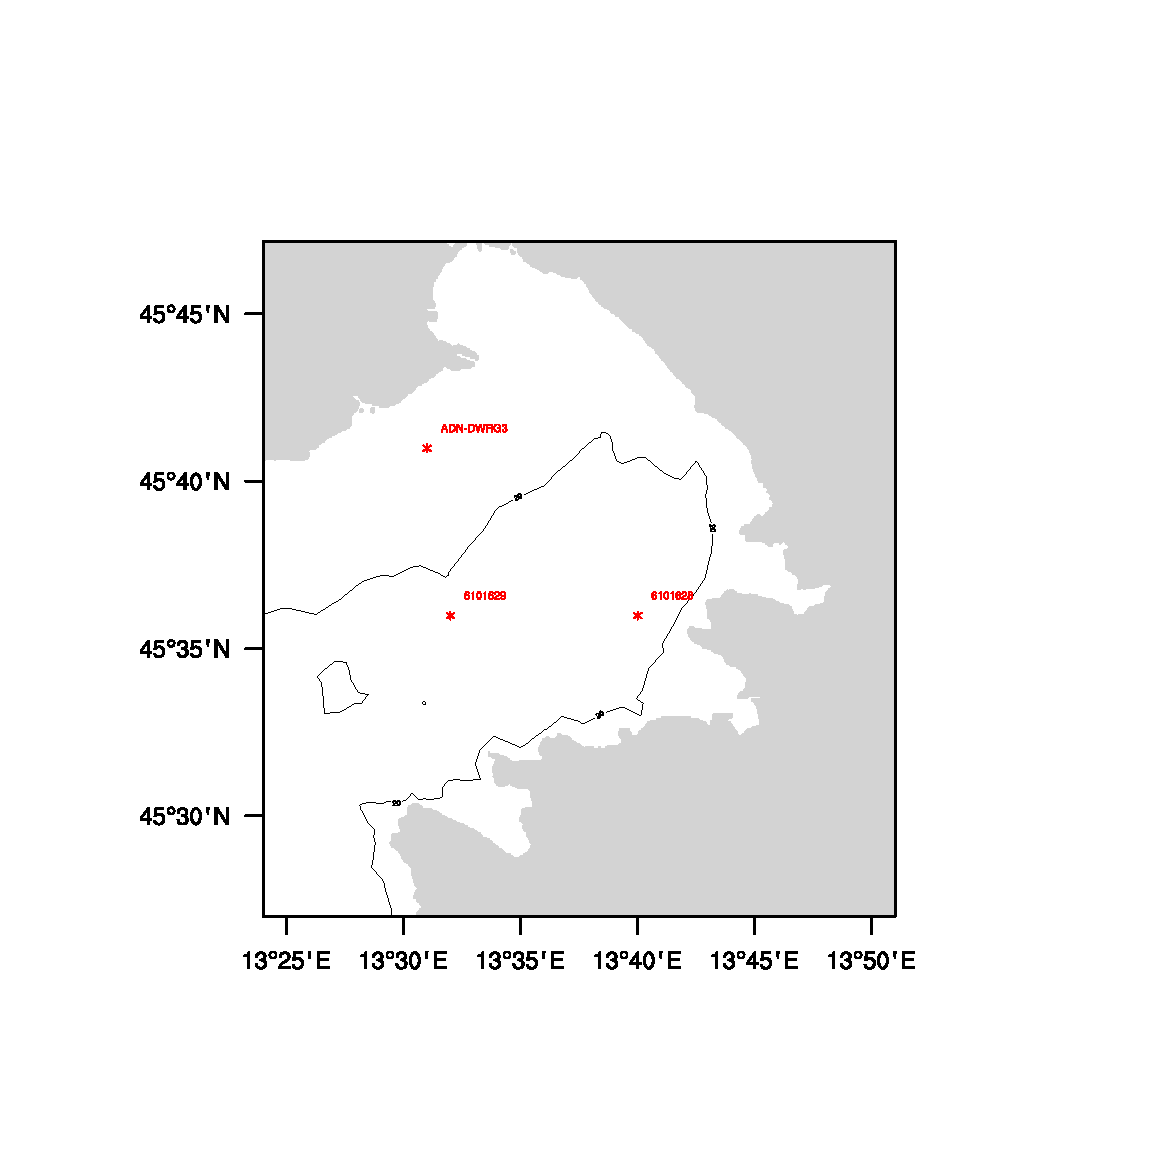
\epsfig{file=Figures_DHMZ_Wave_Paper/MainFIGradar/trimesh.pdf, angle=0, height=4.3cm}\par
\end{minipage}
\begin{minipage}{5.1cm}
\centering
\epsfig{file=Figures_DHMZ_Wave_Paper/WAVE_RADAR_Version1_RUN10_B/Correlation_iGrid0_hs-crop.pdf, height=4.3cm}\par
\end{minipage}
\begin{minipage}{5.1cm}
\centering
\epsfig{file=Figures_DHMZ_Wave_Paper/WAVE_RADAR_Version1_RUN10_B/MeanError_iGrid0_hs-crop.pdf, height=4.3cm}\par
\end{minipage}
\begin{minipage}{5.1cm}
\centering
\epsfig{file=Figures_DHMZ_Wave_Paper/WAVE_RADAR_Version1_RUN10_B/RMSE_iGrid0_hs-crop.pdf, height=4.3cm}\par
\end{minipage}
\end{center}
}


\frame{
  \frametitle{Wave stations I}

\begin{center}
\begin{minipage}{8.1cm}
\centering
\epsfig{file=Figures_DHMZ_Wave_Paper/MainFIGstations/trimesh-crop.pdf, angle=0, height=5.3cm}\par
\end{minipage}
\end{center}
}



\frame{
  \frametitle{Wave stations II}

\begin{center}
\begin{minipage}{5.1cm}
\centering
\epsfig{file=Figures_DHMZ_Wave_Paper/Version1_BUOY_RUN10_B/Scatter_1_Hwave-crop.pdf, height=4.3cm}\par
\end{minipage}
\begin{minipage}{5.1cm}
\centering
\epsfig{file=Figures_DHMZ_Wave_Paper/Version1_BUOY_RUN10_B/Scatter_2_Hwave-crop.pdf, height=4.3cm}\par
\end{minipage}
\begin{minipage}{5.1cm}
\centering
\epsfig{file=Figures_DHMZ_Wave_Paper/Version1_BUOY_RUN10_B/Scatter_3_Hwave-crop.pdf, height=4.3cm}\par
\end{minipage}
\begin{minipage}{5.1cm}
\centering
\epsfig{file=Figures_DHMZ_Wave_Paper/Version1_BUOY_RUN10_B/Scatter_4_Hwave-crop.pdf, height=4.3cm}\par
\end{minipage}
\end{center}

}



\frame{
  \frametitle{Bora event from 2016-11-27 23:00 to 2016-11-30 14:00}

\begin{center}
\begin{minipage}{5.1cm}
\centering
\epsfig{file=Figures_DHMZ_Wave_Paper/PLOT_SINGLE_WIND_bora6_11_28_1900_B/WIND10_0000_20161128_190000-crop.pdf, angle=0, height=4.3cm}\par
\end{minipage}
\begin{minipage}{5.1cm}
\centering
\epsfig{file=Figures_DHMZ_Wave_Paper/PLOT_SINGLE_HS_bora6_11_28_1900/Hwave_0000_20161128_190000-crop.pdf, angle=0, height=4.3cm}\par
\end{minipage}
\begin{minipage}{5.1cm}
\centering
\epsfig{file=Figures_DHMZ_Wave_Paper/PLOT_ALTIMETRY_bora6_11_28_1900/SARAL_Wave_Track0002_at_20161130_042348-crop.pdf, angle=0, height=4.3cm}\par
\end{minipage}
\begin{minipage}{5.1cm}
\centering
\epsfig{file=Figures_DHMZ_Wave_Paper/PLOT_TIMESERIES_bora6_11_28_1900/TimeSeries_iBuoy4_iBlock0_Hwave-crop.pdf, angle=0, height=4.3cm}\par
\end{minipage}
\end{center}
}


\frame{
  \frametitle{Sirocco event from 2016-02-27 05:00 to 2016-02-29 05:00}

\begin{center}
\begin{minipage}{5.1cm}
\centering
\epsfig{file=Figures_DHMZ_Wave_Paper/PLOT_SINGLE_WIND_sirocco2_02_28_2000/WIND10_0000_20160228_200000-crop.pdf, angle=0, height=4.3cm}\par
\end{minipage}
\begin{minipage}{5.1cm}
\centering
\epsfig{file=Figures_DHMZ_Wave_Paper/PLOT_SINGLE_HS_sirocco2_02_28_2000/Hwave_0000_20160228_200000-crop.pdf, angle=0, height=4.3cm}\par
\end{minipage}
\begin{minipage}{5.1cm}
\centering
\epsfig{file=Figures_DHMZ_Wave_Paper/PLOT_ALTIMETRY_sirocco2_saral_02_27/SARAL_Wave_Track0000_at_20160227_174106-crop.pdf, angle=0, height=4.3cm}\par
\end{minipage}
\begin{minipage}{5.1cm}
\centering
\epsfig{file=Figures_DHMZ_Wave_Paper/PLOT_TIMESERIES_sirocco2_02_28_2000/TimeSeries_iBuoy4_iBlock0_Hwave-crop.pdf, angle=0, height=4.3cm}\par
\end{minipage}
\end{center}

}  



\frame{
  \frametitle{Perspectives}

\begin{itemize}
\item Further improvement is needed!
\item Biggest problem is underestimate of wind speed. It is a systematic problem in the Adriatic and near to the sea.\\
Possibilities is to use 4km wind or correcting systematically for the error.
\item Coupling between the atmospheric model ALADIN and the wave model can result if better resolution to the surface layer.
\item Coupling between waves and the circulation model can help in some cases.
\end{itemize}

}




\end{document}
